%===
% SUBSECTION: A different approach taken from nuclear physics
%===
\vspace{7px}
\subsection{A recursive expression for phase space integrals}\label{subsec:recursive-relation}
The following regurgitates parts of~\cite{Byckling:1969sx,Isaacson:2021xty}.
The problem I ran into at the end of the last section was how to use the energy-momentum delta functions to restrict the bounds of integration. Ref.~\cite{Byckling:1969sx} provides a means to circumvent this problem by performing a change of variables. 
Consider the phase space integral $R_n(p_a + p_b)$ defined by (where $p_i$ now denotes a four-momentum vector in constrast to the previous section where it represented a three-momentum magnitude.)
\begin{align}
    R_n(p_a + p_b) = 
    \int \cdots \int \prod_{i=1}^{n} \delta (p_i^2 - m_i^2) \, \Theta(p_i^0) \, 
    \dd^4 p_i \, \delta^4(p_a + p_b - p_1 - \cdots - p_n).
\end{align}
This is manifestly Lorentz invariant and therefore $R_n$ may only be a function of $s \equiv (p_a + p_b)^2$. 
Define the new integration variable $M_{n-1}^2 \equiv (p_a + p_b - p_n)^2$. The physical significance of $M_{n-1}$ is that it is the invariant mass of the first $n-1$ particles, which can be seen using four-momentum conservation: $p_a + p_b - p_n = p_1 + p_2 + \cdots + p_{n-1}$.
It is possible to show that the following recursive relation holds (eqn. (3) of \cite{Byckling:1969sx})
\begin{align}
    \label{eq:recursive-phase-space-relation}
    R_n(s) = 
    \int_{(m_1 + m_2 + \cdots + m_{n-1})^2}^{(\sqrt{s} - m_n)^2} 
    \dd M^2_{n-1} \, \int \dd \Omega_n
    \frac{\sqrt{\lambda(s, M_{n-1}^2, m_n^2)}}{8s} R_{n-1}(M_{n-1}^2)
\end{align}
where $\lambda(x, y, z) = x^2 + y^2 + z^2 - 2 xy - 2 xz - 2yz$ and the solid angle $\dd \Omega_n \equiv \dd \cos \theta_n\, \dd \varphi_n$ defines the direction of $\bm{p}_n$ in the frame where $p_a + p_b = (\sqrt{s}, \bm{0})$. 
The upper limit is obtained by requiring that 
\begin{align}
    |\bm{p}_n|^2 = \frac{\lambda(s, M_{n-1}^2, m_n^2)}{4 s}
\end{align}
be positive whereas the lower limit is threshold below which $R_{n-1}(M_{n-1}^2) = 0$\footnotemark. 
Repeated application of \eref{eq:recursive-phase-space-relation} yields 
\begin{equation}
\begin{aligned}
    R_n&(s) 
        = 
    \int_{(m_1 + m_2 + \cdots + m_{n-1})^2}^{(\sqrt{s} - m_n)^2}
    \dd M^2_{n-1} \,  \int \dd \Omega_n
    \frac{\sqrt{\lambda(s, M_{n-1}^2, m_n^2)}}{8s} \\
        &\times 
    \int_{(m_1 + m_2 + \cdots + m_{n-2})^2}^{(M_{n-1} - m_{n-1})^2}
    \dd M^2_{n-2}  \, \int \dd \Omega_{n-1}
    \frac{\sqrt{\lambda(M_{n-1}^2, M_{n-2}^2, m_{n-1}^2)}}{8M_{n-1}^2} \\
        &\times \cdots \times
    \int_{(m_1 + m_2)^2}^{(M_3 - m_3)^2}
    \dd M^2_{2}  \, \int \dd \Omega_{3}
    \frac{\sqrt{\lambda(M_{3}^2, M_{2}^2, m_{3}^2)}}{8M_{3}^2} 
    \times 
    \int \dd \Omega_2
    \frac{\sqrt{\lambda(M_{2}^2, m_1^2, m_{2}^2)}}{8M_{2}^2}. 
\end{aligned}
\end{equation}

% WHICH IS MORE USEFUL TO SHOW? N = 3 OR N = 5? PROBABLY N =5.
The important case for me is $n = 3$:
\begin{equation}
\begin{aligned}
    R_3(s) = 
        \int_{(m_1 + m_2)^2}^{(\sqrt{s} - m_3)^2} \dd M_{2}^2 
        \int \dd \Omega_3 \,
        \frac{\lambda (s, M^2_{2}, m_3^2)}{8s} \,
        \int \dd \Omega_2 \,
        \frac{\lambda (M^2_2, m_1^2, m_2^2)}{8 M_2^2} \; .
\end{aligned}
\end{equation}
It's easy to verify that the number of integration variables matches our expectation of $3(3) - 4 = 5$ since we are integrating over one invariant mass, and two pairs of two angles. 

In the above discussion we have considered $p_a$ and $p_b$ to be fixed.
However, for my purposes I will also be integrating over $p_a$ and $p_b$.
This case seems to be similar to the one considered in~\cite{Isaacson:2021xty} (cf. the example given between their eqs. (12) and (13)).
% Since we are integrating over both ingoing and outgoing momenta we need the formula for $n = 5$ with $s = 0$. This is because in our case we have a $\delta$ function of the form $\delta^4(p_a + p_b - p_1 - p_2 - p_3)$ but we are also integrating over $p_a$ and $p_b$. Relabel $p_a \rightarrow - k_1$, $p_b \rightarrow - k_2$, and $p_i \rightarrow k_{i + 2}$. Then,
% \begin{align*}
%     \delta^4(p_a + p_b - p_1 - p_2 - p_3) \rightarrow \delta^4(0 - k_1 - k_2 - k_3 - k_4 - k_5)
% \end{align*}
% which motivates the need for $R_n(s = 0)$.
% \begin{equation}
% \begin{aligned}
%     R_5(s) = 
%         & \int_{(m_1 + m_2 + m_3 + m_4)^2}^{(\sqrt{s} - m_4)^2} \dd M_{4}^2 
%             \int \dd \Omega_5 \,
%             \frac{\sqrt{\lambda (s, M^2_{4}, m_5^2)}}{8s} \\
%         & \times 
%             \int_{(m_1 + m_2 + m_3)^2}^{(M_4 - m_4)^2} \dd M_{3}^2 
%             \int \dd \Omega_4 \,
%             \frac{\sqrt{\lambda (M^2_4, M^2_3, m_4)}}{8 M^2_4} \\
%         & \times
%             \int_{(m_1 + m_2)^2}^{(M_3 - m_3)^2} \dd M_{2}^2 
%             \int \dd \Omega_3 \,
%             \frac{\sqrt{\lambda (M^2_3, M^2_2, m_3)}}{8 M^2_3}
%             \int \dd \Omega_2 \,
%             \frac{\sqrt{\lambda (M^2_2, m_1^2, m_2^2)}}{8 M_2^2} \; .
% \end{aligned}
% \end{equation}

\footnotetext{In eq. (3) of~\cite{Byckling:1969sx} the authors allude that the angular $\dd \Omega$ integrals can be performed. They do not perform the integrals because \emph{``the variables defining a momentum vector should appear explicitly if a Monte Carlo method is to be applied for the generation of events.''} In my case I think that we still can't do these integrals trivially because the matrix element depends on them, although I'm not 100\% sure if this is correct.}

\begin{figure}[t]
    \centering
    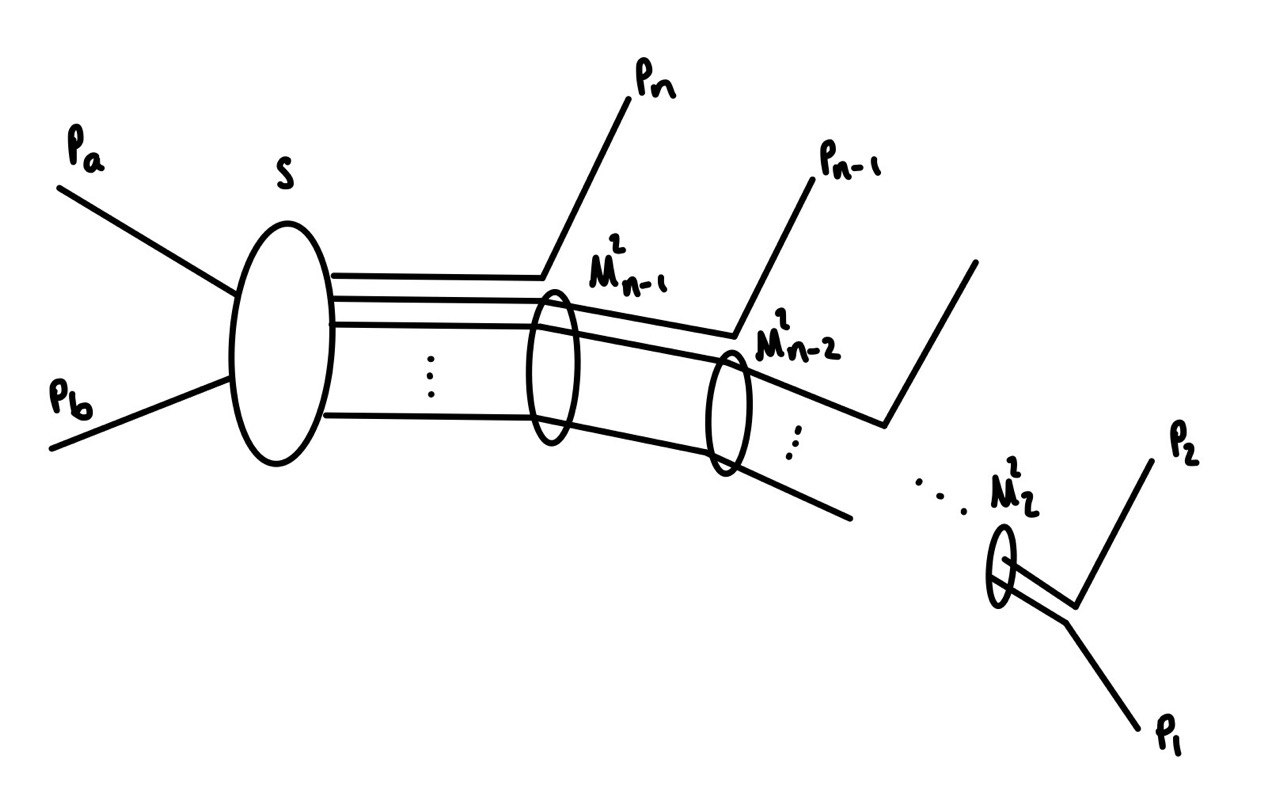
\includegraphics[width=0.6\linewidth]{figs/recursion-diagram.jpg}
    \caption{Illustration of the recursion relation as a sequence of effective $2 \rightarrow 2$ scattering events.}
    \label{fig:recursion-diagram}
\end{figure}

%====
% SUBSECTION: Writing the integral in terms of momentum transfers 
%====
\vspace{7px}
\subsection{Writing integral in terms of momentum transfers}\label{subsec:momentum-transfers}

In sec~\ref{subsec:recursive-relation} we wrote the phase space integral in terms of invariant masses and angles of the three-momenta $\bm{p}_i$ defined in the center-of-mass frame where $\sum_{k=1}^{i} p_k = (M_{i}, \bm{0})$. 
The matrix element in \eref{eq:matrix-element} is a function of the Lorentz invariants $(p_a \cdot p_1), \; (p_b \cdot p_3), \; (p_2 \cdot p_3)$, and $(p_b \cdot p_2) = (- (p_a - p_1 - p_2 - p_3) \cdot p_2)$. 
It is cumbersome to write this matrix element explicitly in terms of the angles $\{ (\theta_i, \varphi_i) : i = 1, 2, \ldots, n\}$ so we would rather use kinematic Lorentz invariants analogous to the Mandelstam variables for $2 \rightarrow 2$ scattering.
To this end it is convenient to introduce the so-called `momentum transfers' $t_i \equiv Q_i^2 \equiv (p_a - p_1 - \cdots - p_i)^2 = (p_n + p_{n-1} + \cdots + p_{i + 1} - p_b)^2$.

Some of the dot products may be written exclusively in terms of the kinematic variables. For example,
\begin{gather*}
    \begin{align*}
        t_1 &\equiv (p_a - p_1)^2 &&\rightarrow &&2 p_a \cdot p_1 = m_a^2 +  m_1^2 - t_1 \\
        t_2 &\equiv (p_a - (p_1 + p_2))^2 &&\rightarrow &&2 p_a \cdot p_2 = M_2^2 - m_1^2 + t_1 - t_2 \\
        t_3 &\equiv (p_a - (p_1 + p_2 + p_3))^2 &&\rightarrow &&2 p_a \cdot p_3 = M_3^2 - M_2^2 + t_2 \\
        M_2^2 &\equiv (p_1 + p_2)^2 &&\rightarrow &&2 p_1 \cdot p_2 = M_2^2 - m_1^2 - m_2^2 \\
        M_3^2 &\equiv (p_1 + p_2 + p_3)^2 &&\rightarrow &&2 (p_1 + p_2) \cdot p_3 = M_3^2 - 2 M_2^2 + m_1^2 + m_2^2 - m_3^2 \\
    \end{align*}
\end{gather*}
However I was unable to write $p_2 \cdot p_3$ in terms of the invariants alone. 
$p_b \cdot p_2$ is really just $p_2 \cdot p_3$ in disguise so it has the same problem.
I believe this is because these variables are not enough to fully describe the system and some angles are required in addition. 
We need $3(3) - 4 = 5$ integration variables but only $3$ of them are prescribed by the kinematic invariants $M_2^2$, $t_1$, and $t_2$\footnotemark.
I haven't followed their derivation through in enough detail to understand precisely how they show up in the expression 
\todo{
    Understand how to write the matrix element explicitly in terms of the angles $\varphi_1$, $\varphi_2$ as well as the invariants $M_2^2$, $t_1$, and $t_2$.
}.

The two additional degrees of freedom can be seen in eq. (14) of~\cite{Byckling:1969sx}. 
They are the azimuthal angles $\varphi_1$, $\varphi_2$ as seen in a frame where $p_a = (m_a, \bm{0})$.   

\footnotetext{$M_1^2 = m_1^2$,  $M_3^2 = s$ and  $t_3 = (-p_b)^2 = m_b^2$ are all constants, not integration variables.}  